\documentclass{standalone}
\usepackage{tikz}
\usepackage{mathpazo}
\begin{document}
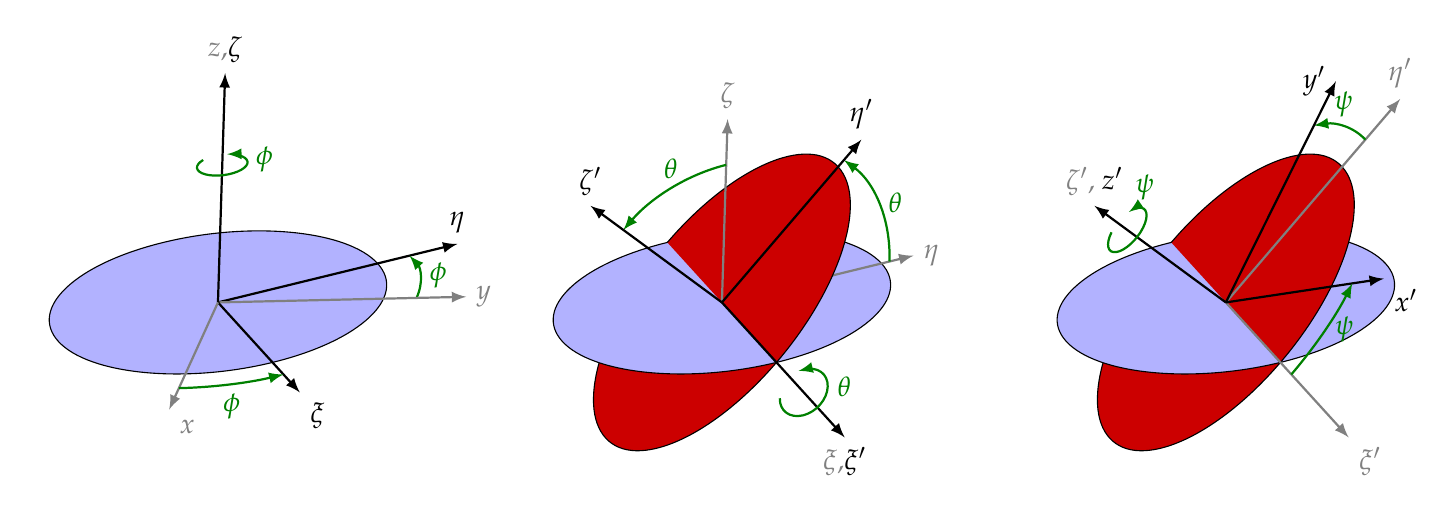
\begin{tikzpicture}

% ======= GENERAL PARAMETERS =======
\def\radius{2}          % Base sphere radius
\def\rA{0.3}            % Small arc radius (for angle indicators)
\def\addAx{1}           % Extra axis length for arrows
\def\nutation{45}       % Nutation angle 
\def\precession{-30}    % Precession angle 

% =====================================================
% ================ FIGURE 1: BASE SYSTEM ===============
% =====================================================
% (Shifted left for layout)
\begin{scope}[shift={(-3.2*\radius,0)}]
  % Rotate the scene for a 3D-like view
  \begin{scope}[rotate around y =-50, rotate around x = -90, rotate around y = 5]
  
    % --- Draw base sphere (blue) ---
    \draw[fill=blue!30] (0,0) circle (\radius);
    
    % --- Fixed vertical axis (eta) ---
    \draw[thick, -latex] (0,0,0) -- (0,\radius+\addAx,0) node[above] {$\eta$};

    % --- Precession arc (phi) around z-axis ---
    \draw[thick, latex-, color=green!50!black] (0,0) ++(90:\radius+0.4) arc (90:90+\precession:\radius+0.4);
    \path (0,0) ++(90:\radius+0.4) arc (90:90+0.5*\precession:\radius+0.4) node[right]{\textcolor{green!50!black}{$\phi$}};

    % --- Coordinate axes: y, z, xi ---
    \draw[thick, -latex, color=gray] (0,0,0) -- (90+\precession:\radius+\addAx) node[right] {$y$};
    \draw[thick, -latex] (0,0,0) -- (0,0,\radius+\addAx) node[above] {\textcolor{gray}{$z,$}$\zeta$};
    \draw[thick, -latex] (0,0,0) -- (\radius+\addAx,0,0) node[below right] {$\xi$};

    % --- Small arc near top to indicate phi angle ---
    \begin{scope}[shift={(0,0,0.9*\radius)}]
      \draw[thick, -latex, color=green!50!black] (0,0) ++(-150:\rA) arc(-150:150:\rA);
      \path (0,0) ++(-150:\rA) arc(-150:90:\rA) node[right]{\textcolor{green!50!black}{$\phi$}};
    \end{scope}

    % --- Rotated x-axis (after precession) ---
    \begin{scope}[rotate around z = \precession]
      \draw[thick, -latex,color=gray] (0,0,0) -- (\radius+\addAx,0,0) node[below right] {$x$};
    \end{scope}

    % --- Draw phi arc between xi and x axes ---
    \draw[thick,latex-, color=green!50!black] (0,0) ++(\radius+0.4,0,0) arc (0:\precession:\radius+0.4);
    \path (0,0) ++(\radius+0.4,0,0) arc (0:0.5*\precession:\radius+0.4) node[below] {\textcolor{green!50!black}{$\phi$}};

  \end{scope}
\end{scope}


% =====================================================
% ================ FIGURE 2: ADD NUTATION ==============
% =====================================================
\begin{scope}[rotate around y =-50, rotate around x = -90, rotate around y = 5]

  % --- tilted circle: plane after nutation ---
  \begin{scope}[rotate around x = \nutation]
    \draw[fill=red!80!black] (0,0,0) -- (-\radius,0,0 ) arc (180:360:\radius);
  \end{scope}

  % --- Blue base circle (reference plane) ---
  \draw[fill=blue!30] (0,0) circle (\radius);

  % --- eta axis (vertical) ---
  \draw[thick, -latex, color=gray] (0,0,0) -- (0,\radius+0.4,0) node[right] {$\eta$};

  % --- tilted circle (bottom half) for nutation visualization ---
  \begin{scope}[rotate around x = \nutation]
    \draw[fill=red!80!black] (0,0,0) -- (\radius,0,0 ) arc (0:180:\radius);
  \end{scope}

  % --- Main axes: z and xi′ ---
  \draw[thick, -latex, color=gray] (0,0,0) -- (0,0,\radius+0.4) node[above] {$\zeta$};
  \draw[thick, -latex] (0,0,0) -- (\radius+2.5,0,0) node[below] {\textcolor{gray}{$\xi,$}$\xi'$};

  % --- Small arc showing nutation angle theta near right side ---
  \begin{scope}[shift={(\radius+1,0,0)}]
    \begin{scope}[rotate around y=90]
      \draw[thick, -latex, color=green!50!black] (0,0) ++(-90:\rA) arc(-90:180:\rA) -- ++(0,-0.075,0);
      \node[right] at (0,\rA,0) {\textcolor{green!50!black}{$\theta$}};
    \end{scope}
  \end{scope}

  % --- theta arcs showing tilt between z and z′ ---
  \begin{scope}[rotate around y=90]
    \draw[thick,-latex, color=green!50!black] (0,0,0) ++(90:\radius+0.1)  arc (90:90+\nutation:\radius+0.1);
    \path (0,0,0) ++(90:\radius+0.1)  arc (90:90+0.5*\nutation:\radius+0.1) node[right] {\textcolor{green!50!black}{$\theta$}};

    \draw[thick,-latex,color=green!50!black] (0,0,0) ++(180:\radius-0.2)  arc (180:180+\nutation:\radius-0.2);
    \path (0,0,0) ++(180:\radius-0.2)  arc (180:180+0.5*\nutation:\radius-0.2) node[above] {\textcolor{green!50!black}{$\theta$}};

    % --- Tilted axes after nutation ---
    \draw[thick,-latex] (0,0) -- (180+\nutation:\radius+0.4) node[above] {$\zeta'$};
    \draw[thick,-latex] (0,0) -- (90+\nutation:\radius+0.4) node[above] {$\eta'$};
  \end{scope}

  % % --- x-axis rotated by precession phi ---
  % \begin{scope}[rotate around z = \precession]
  %   \draw[thick, -latex, color=gray] (0,0,0) -- (\radius+\addAx,0,0) node[below right] {$x$};
  % \end{scope}

  % % --- phi arc again (for reference) ---
  % \draw[thick,dashed,latex-, color=gray] (0,0) ++(\radius-0.2,0,0) arc (0:\precession:\radius-0.2);
  % \path (0,0) ++(\radius-0.2,0,0) arc (0:0.5*\precession:\radius-0.2) node[below] {\textcolor{gray}{$\phi$}};
\end{scope}


% =====================================================
% ================ FIGURE 3: ADD SPIN =================
% =====================================================
\begin{scope}[shift={(3.2*\radius,0)}]
  \begin{scope}[rotate around y =-50, rotate around x = -90, rotate around y = 5]

    % --- Same as figure 2: tilted red!80!black and base blue circles ---
    \begin{scope}[rotate around x = \nutation]
      \draw[fill=red!80!black] (0,0,0) -- (-\radius,0,0 ) arc (180:360:\radius);
    \end{scope}
    \draw[fill=blue!30] (0,0) circle (\radius);
    % \draw[thick, -latex,color=gray] (0,0,0) -- (0,\radius+0.4,0) node[right] {$\eta$};

    \begin{scope}[rotate around x = \nutation]
      \draw[fill=red!80!black] (0,0,0) -- (\radius,0,0 ) arc (0:180:\radius);
    \end{scope}

    % --- Axes y, z, xi′ ---
    % \draw[thick, -latex,color=gray] (0,0,0) -- (0,0,\radius+0.4) node[above] {$z$};
    % \draw[thick, -latex, color=gray] (0,0,0) -- (90+\precession:\radius+\addAx) node[right] {$y$};
    \draw[thick, -latex,color=gray] (0,0,0) -- (\radius+2.5,0,0) node[below right] {$\xi'$};

    % --- Arc for nutation theta ---
    % \begin{scope}[rotate around y=90]
    %   \draw[thick,-latex] (0,0,0) ++(90:\radius+0.1)  arc (90:90+\nutation:\radius+0.1);
    %   \path (0,0,0) ++(90:\radius+0.1)  arc (90:90+0.5*\nutation:\radius+0.1) node[right] {$\theta$};
    % \end{scope}

    % --- x-axis rotated by precession phi ---
    % \begin{scope}[rotate around z = \precession]
    %   \draw[thick, -latex] (0,0,0) -- (\radius+\addAx,0,0) node[below right] {$x$};
    % \end{scope}

    % --- phi arc for reference ---
    % \draw[thick,latex-] (0,0) ++(\radius+0.4,0,0) arc (0:\precession:\radius+0.4);
    % \path (0,0) ++(\radius+0.4,0,0) arc (0:0.5*\precession:\radius+0.4) node[below] {$\phi$};
  \end{scope}

  % -----------------------------------------------------
  % ADDITIONAL ELEMENTS for FIGURE 3 (Spin phi)
  % -----------------------------------------------------
  \begin{scope}[rotate around y =-50, rotate around x = -90, rotate around y = 5]

    % --- Axes of rotated body frame after nutation ---
    \begin{scope}[rotate around x = \nutation]
      \draw[thick, -latex,color=gray] (0,0,0) -- (0,\radius+1,0) node[above] {$\eta'$};

      % --- psi precession (spin) arc around eta' ---
      \draw[thick, -latex,color=green!50!black] (0,0) ++(90:\radius+0.4) arc (90:90-\precession:\radius+0.4);
      \path (0,0) ++(90:\radius+0.4) arc (90:90-0.5*\precession:\radius+0.4) node[above]{\textcolor{green!50!black}{$\psi$}};

      % --- Axes after psi rotation (body frame) ---
      \draw[thick, -latex] (0,0,0) -- (90-\precession:\radius+1) node[left] {$y'$};
      \draw[thick, -latex] (0,0,0) -- (0,0,\radius+0.4) node[above] {\textcolor{gray}{$\zeta'$, }$z'$};

      % --- Small psi arc marker on top ---
      \begin{scope}[shift={(0,0,0.9*\radius)}]
        \draw[thick, -latex, color=green!50!black] (0,0) ++(-150:\rA) arc(-150:150:\rA);
        \path (0,0) ++(90:\rA) node[align=left,above]{\textcolor{green!50!black}{$\psi$}};
      \end{scope}

      % --- x′ axis (rotated by psi) ---
      \begin{scope}[rotate around z = -\precession]
        \draw[thick, -latex] (0,0,0) -- (\radius+1,0,0) node[below right] {$x'$};
      \end{scope}

      % --- psi arc indicator between xi′ and x′ ---
      \draw[thick,-latex,color=green!50!black] (0,0) ++(\radius+0.4,0,0) arc (0:-\precession:\radius+0.4);
      \path (0,0) ++(\radius+0.4,0,0) arc (0:-0.5*\precession:\radius+0.4) node[right] {\textcolor{green!50!black}{$\psi$}};
    \end{scope}
  \end{scope}
\end{scope}

\end{tikzpicture}
\end{document}
